\section{Introduction}
\label{sec:introduction}

Suppose~$U$ is a universe of \textit{keys}.
Let $h:U\to M$ be a {\em hash function} that maps the keys from~$U$
to a given interval of integers $M=[0,m-1]=\{0,1,\dots,m-1\}$.
Let~$S\subseteq U$ be a set of~$n$ keys from~$U$.
Given a key~$x\in S$, the hash function~$h$ computes an integer in
$[0,m-1]$ for the storage or retrieval of~$x$ in a {\em hash table}.
Hashing methods for {\em non-static sets} of keys can be used to construct
data structures storing $S$ and supporting membership queries
``$x \in S$?'' in expected time $O(1)$.
However, they involve a certain amount of wasted space owing to unused
locations in the table and waisted time to resolve collisions when
two keys are hashed to the same table location.

For {\em static sets} of keys it is possible to compute a function
to find any key in a table in one probe; such hash functions are called
\textit{perfect}. 
Given a set of keys~$S$, we shall say that a hash function~$h:U\to M$ is a
\textit{perfect hash function} for~$S$ if~$h$ is an injection on~$S$,
that is, there are no \textit{collisions} among the keys in~$S$: if~$x$
and~$y$ are in~$S$ and~$x\neq y$, then~$h(x)\neq h(y)$.
Figure~\ref{fig:minimalperfecthash-ph-mph}(a) illustrates a perfect hash
function.
Since no collisions occur, each key can be retrieved from the table
with a single probe.
If~$m=n$, that is, the table has the same size as~$S$,
then~$h$ is a \textit{minimal perfect hash function} for~$S$.
Figure~\ref{fig:minimalperfecthash-ph-mph}(b) illustrates
a~minimal perfect hash function.
Minimal perfect hash functions totally avoid the problem of wasted
space and time.

% For two-column wide figures use
\begin{figure*}
% Use the relevant command to insert your figure file.
% For example, with the graphicx package use
\centering
  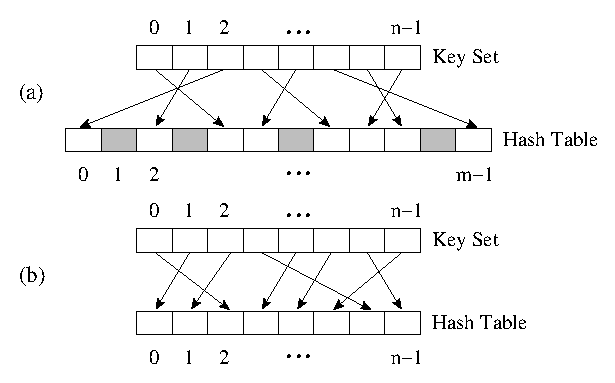
\includegraphics{figs/minimalperfecthash-ph-mph.ps}
% figure caption is below the figure
\caption{(a) Perfect hash function\quad  (b) Minimal perfect hash function}
\label{fig:minimalperfecthash-ph-mph}
\end{figure*}

Minimal perfect hash functions are widely used for memory efficient
storage
and fast retrieval of items from static sets, such as words in natural
languages, reserved words in programming languages or interactive systems,
universal resource locations (URLs) in Web search engines, or item sets in
data mining techniques.

The aim of this paper is to describe a new way of constructing minimal perfect
hash functions.  Our algorithm shares several features with the one due to
Czech, Havas and Majewski~\cite{chm92}.  In particular, our algorithm is also
based on the generation of random graphs~$G=(V,E)$, where~$E$ is in one-to-one
correspondence with the key set~$S$ for which we wish to generate the hash
function.
The two main differences between our algorithm and theirs
are as follows:
(\textit{i})~we generate random graphs
$G = (V, E)$ with $|V|=cn$ and $|E|=|S|=n$, where~$c=1.15$, and hence~$G$
contains cycles with high probability,
while they generate \textit{acyclic} random graphs
$G = (V, E)$ with $|V|=cn$ and $|E|=|S|=n$,
with a greater number of vertices: $|V|\ge2.09n$;
(\textit{ii})~they generate order preserving minimal perfect hash functions
while our algorithm does not preserve order (a perfect hash function $h$ is
\textit{order preserving} if the keys in~$S$ are arranged in some given order
and~$h$ preserves this order in the hash table).  Thus, our algorithm improves
the space requirement at the expense of generating functions that are not
order preserving.

Our algorithm is efficient and may be tuned to yield a function~$h$
with a very economical description.
As the algorithm in~\cite{chm92}, our algorithm produces~$h$
in~$O(n)$ expected time for a set of~$n$ keys.
The description of~$h$ requires~$1.15n$ computer words,
and evaluating~$h(x)$
requires two accesses to an array of~$1.15n$ integers.
We further derive a heuristic that improves the space requirement
from~$1.15n$ words down to~$0.93n$ words.
Our scheme is very practical: to generate a minimal perfect hash function for
a collection of 100~million universe resource locations (URLs), each 63 bytes
long on average, our algorithm running on a commodity PC takes 811 seconds on
average.
